
Figure \ref{fig:FIGS} shows qualitative results for the Plane-Tree. The third row shows the bunny, rabbit and horse models along with the number of bytes and bpv required to store them uncompressed. The first row shows each model compressed by the Plane-Tree with a threshold of 8.0. Despite these being crude approximations of the originals, the models are still distinguishable with around 1000 $\times$ less storage space required. \\

In the second row, each model was compressed with the Plane-Tree at a threshold of 1.0. In these experiments, there is little detail missing compared with the physical model. When looking at the bunny's legs, the same ripples are present. In the rabbit model, the outlines inside the ears and on the eyes are still present. On the horse model, the creases on the body and shoulder of the horse are still present. Here, the bunny is compressed to around 70 $\times$ less storage space, the rabbit at around 265 $\times$ less and the horse around 90 $\times$ less storage space. \\


\begin{figure*}[!htb] 
        \centering
 		\begin{subfigure}[b]{1.9in}
                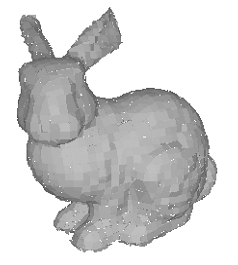
\includegraphics[width=1.6in]{images/results/compression/bunnyb}
                \caption{2.03 bpv\\8827 bytes}
                \label{fig:FIG_BUNNYB}
        \end{subfigure}%
        \begin{subfigure}[b]{1.9in}
                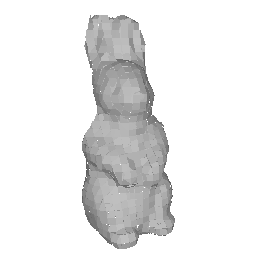
\includegraphics[width=1.6in]{images/results/compression/rabbitb}
                \caption{0.47\\3898 bytes}
                \label{fig:FIG_RABBITB}
        \end{subfigure}%
        \begin{subfigure}[b]{1.9in}
                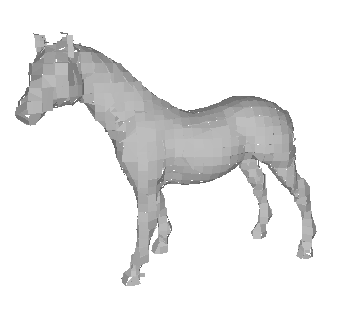
\includegraphics[width=1.6in]{images/results/compression/horseb}
                \caption{1.55 bpv\\3842 bytes}
                \label{fig:FIG_HORSEB}
        \end{subfigure}

        \begin{subfigure}[b]{1.9in}
                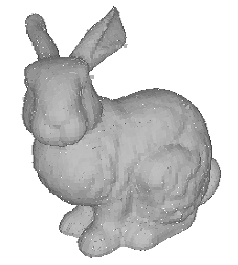
\includegraphics[width=1.6in]{images/results/compression/bunnyd}
                \caption{7.74 bpv\\33701 bytes}
                \label{fig:FIG_BUNNYD}
        \end{subfigure}%
        \begin{subfigure}[b]{1.9in}
                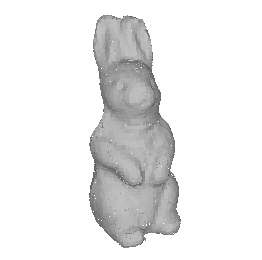
\includegraphics[width=1.6in]{images/results/compression/rabbitd}
                \caption{1.97\\16492 bytes}
                \label{fig:FIG_RABBITD}
        \end{subfigure}%
        \begin{subfigure}[b]{1.9in}
                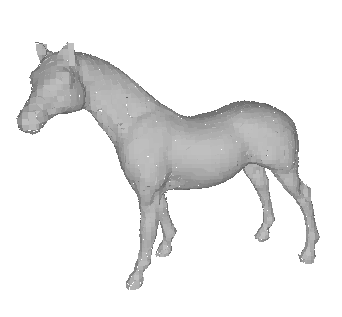
\includegraphics[width=1.6in]{images/results/compression/horsed}
                \caption{5.95 bpv\\14758 bytes}
                \label{fig:FIG_HORSED}
        \end{subfigure}
        
        \begin{subfigure}[b]{1.9in}
                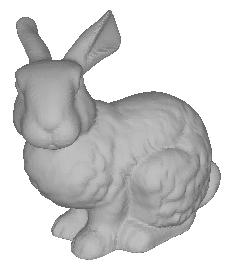
\includegraphics[width=1.6in]{images/results/compression/bunnyorig}
                \caption{original: 518.78 bpv\\2,258,902 bytes}
                \label{fig:FIG_BUNNYO}
        \end{subfigure}%
        \begin{subfigure}[b]{1.9in}
                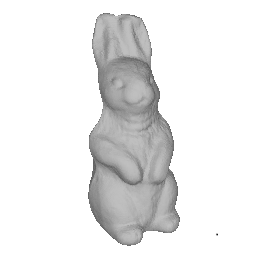
\includegraphics[width=1.6in]{images/results/compression/rabbitorig}
                \caption{original: 530.14\\4,442,413 bytes}
                \label{fig:FIG_RABBITO}
        \end{subfigure}%
        \begin{subfigure}[b]{1.9in}
                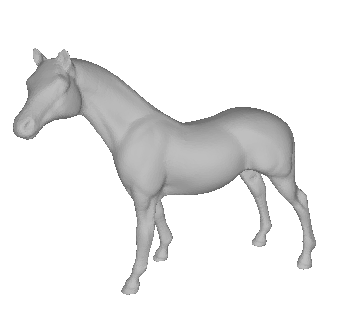
\includegraphics[width=1.6in]{images/results/compression/horseorig}
                \caption{original: 519.92 bpv\\1,290,120 bytes}
                \label{fig:FIG_HORSEO}
        \end{subfigure}
       
       \caption{Models coded with our coder at thresholds of 8.0 and 1.0 with a maximum tree depth of 6 along with the original models.}
       \label{fig:FIGS}
\end{figure*}

Figure \ref{fig:qualSOTA1} shows the Bunny model compressed using the Plane-Tree method and two state-of-the-art methods, the valence method \cite{touma98triangle} and the spectral method \cite{Karni00Spectral}. The original model in Figure \ref{fig:PT_SOTAQ1_ORIG} requires 2,258,902 bytes for storage. The valence method and the spectral method require ~17,852 bytes to store the model and the compression effects are shown in Figures \ref{fig:PT_SOTAQ1_TG} and \ref{fig:PT_SOTAQ1_KG}. Noticeable artefacts not present in the original model are produced by both codecs. The model coded by the valence method fairs worse than the one coded by the spectral method. The model compressed by the Plane-Tree requires just over half the amount of bytes than the other codecs. The Plane-Tree coded model is smoother than the other models (despite flat shading) too. This is likely due to the way the Plane-Tree compression system approximates the original model using planes. This process doesn't introduce these artefacts, allowing the Plane-Tree to represent the original model more accurately. \\   

\begin{figure}[H] 
        \begin{center}
 		\begin{subfigure}[b]{3in}
 			   \centering
 			   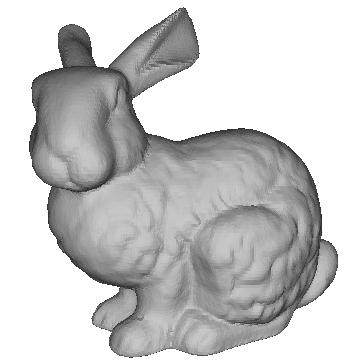
\includegraphics[width=2.8in]{images/experiments/pt_qual/original1}
 			   \captionsetup{justification=centering}
                \caption{Original\\518.78 bpv\\2,258,902 bytes}
                \label{fig:PT_SOTAQ1_ORIG}
        \end{subfigure}%
        \begin{subfigure}[b]{3in}
                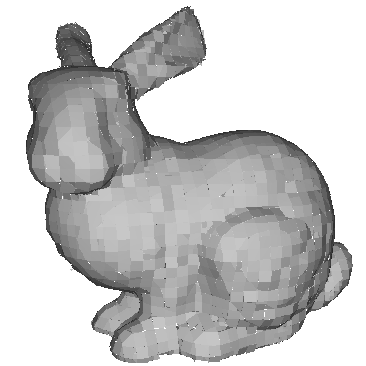
\includegraphics[width=2.8in]{images/experiments/pt_qual/pt_11004}
                \captionsetup{justification=centering}
                \caption{Plane-Tree\\2.52 bpv\\11,003 bytes}
                \label{fig:PT_SOTAQ1_PLT}
        \end{subfigure}
        \begin{subfigure}[b]{3in}
                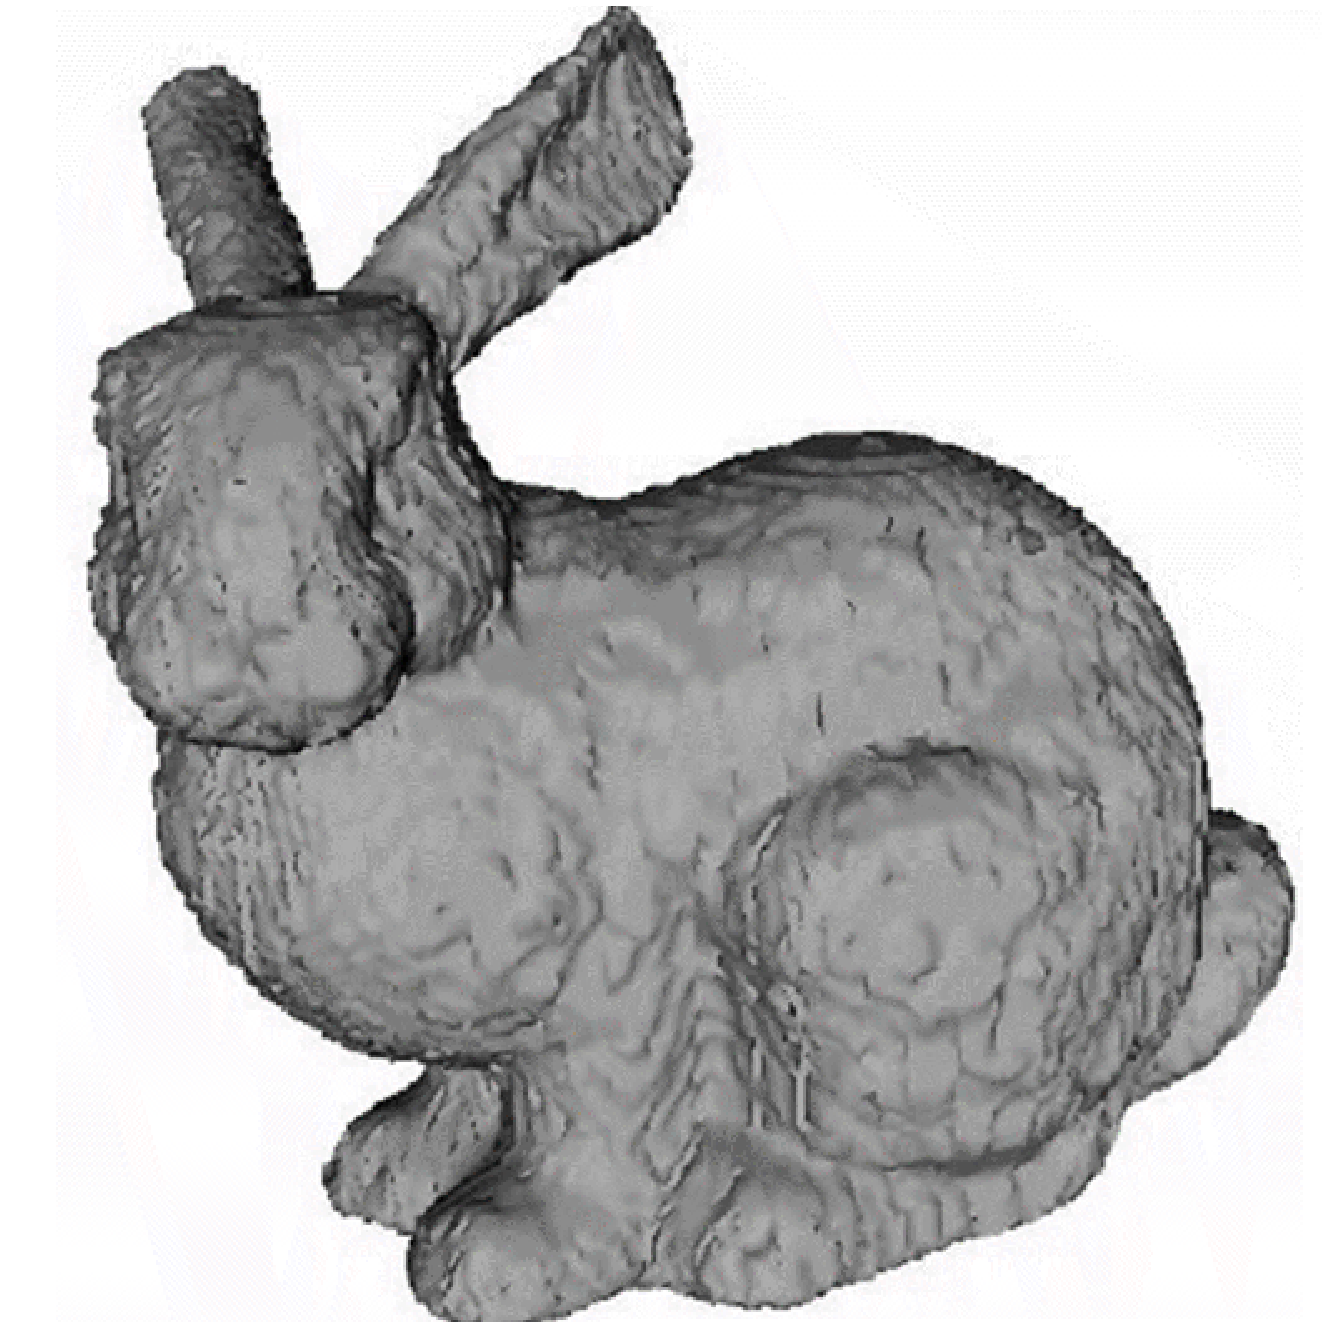
\includegraphics[width=2.8in]{images/experiments/pt_qual/tg}
                \captionsetup{justification=centering}
                \caption{Valence Method \cite{touma98triangle}\\4.1 bpv\\17,852 bytes}
                \label{fig:PT_SOTAQ1_TG}
        \end{subfigure}%
        \begin{subfigure}[b]{3in}
                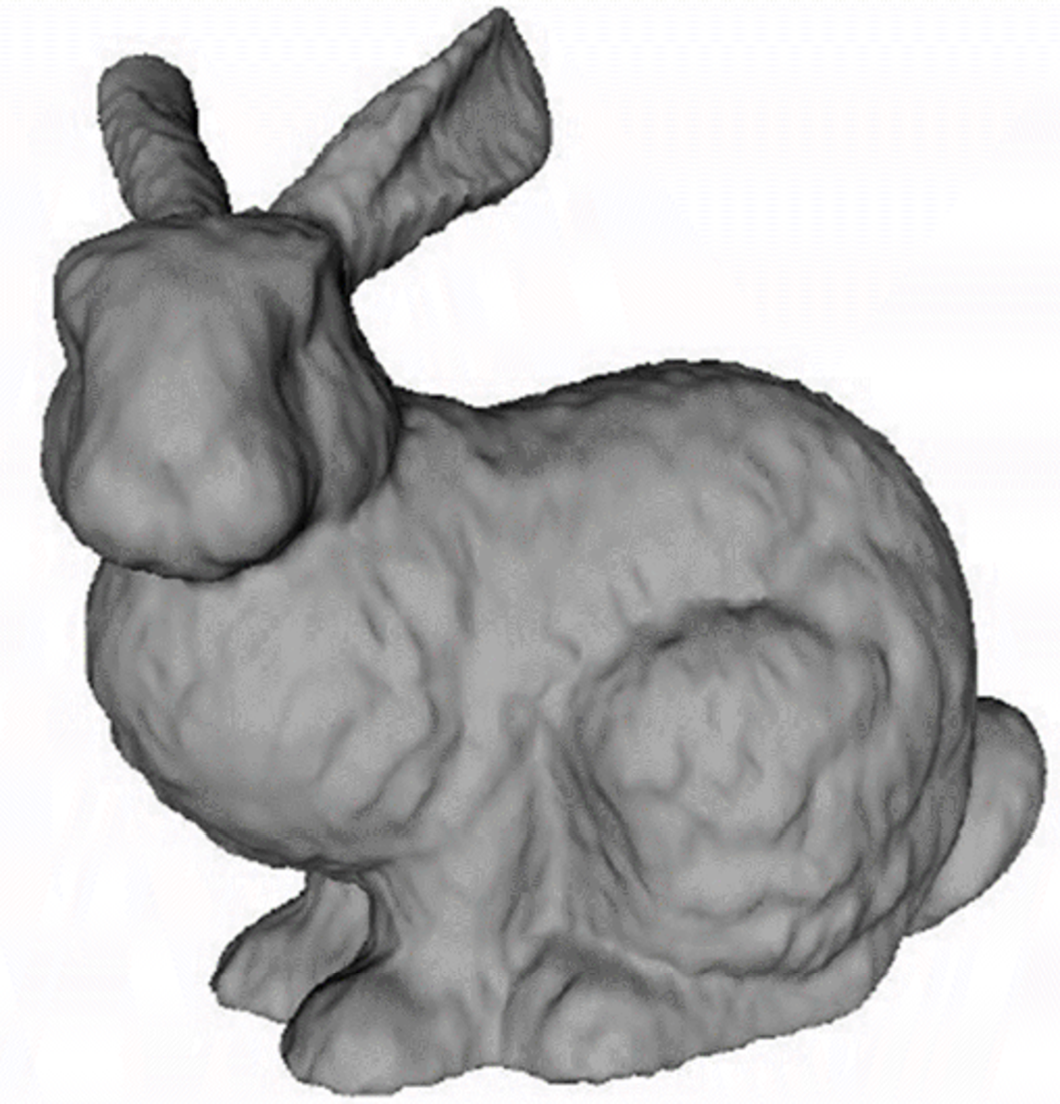
\includegraphics[width=2.8in]{images/experiments/pt_qual/kg}
                \captionsetup{justification=centering}
                \caption{Spectral Method \cite{Karni00Spectral}\\4.1 bpv\\17,852 bytes}
                \label{fig:PT_SOTAQ1_KG}
        \end{subfigure}
       \caption{The Bunny Model Compressed Using the Plane-Tree, Valence and Spectral Methods.}
       \label{fig:qualSOTA1}
       \end{center}
\end{figure}

Figure \ref{fig:qualSOTA2} shows the bunny model coded using the Plane-Tree and the codec by Khodakovsky et al. Both the Plane-Tree and method by Khodakovsky et al. require just 1349 bytes of storage to represent these low bit-rate models. Both methods however, use different strategies and introduce different styles of noise into the compressed model. The method by Khodakovsky et al. shrinks the models and warps the shape, simplifying it. The Plane-tree approximates the shape and positions of the vertices more closely but does not produce smooth surfaces. We conclude that both methods may be beneficial in different situations. The method by Khodakovsky et al. may be useful in situations where visual appeal are important. The Plane-Tree method may be more useful in applications where model shape and size are more important. \\

\begin{figure}[H] 
        \begin{center}
 		\begin{subfigure}[b]{2in}
 			   \centering
 			   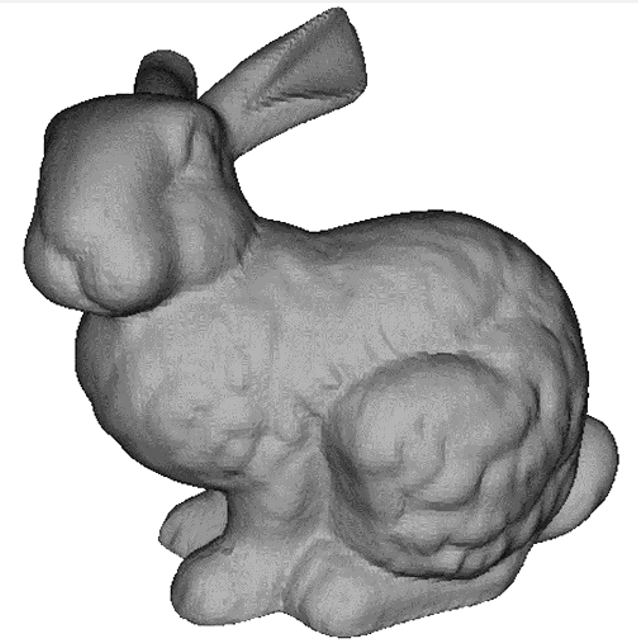
\includegraphics[width=1.8in]{images/experiments/pt_qual/original2}
				\captionsetup{justification=centering}
                \caption{Original\\518.78 bpv\\2,258,902 bytes}
                \label{fig:PT_SOTAQ2_ORIG}
        \end{subfigure}%
        \begin{subfigure}[b]{2in}
                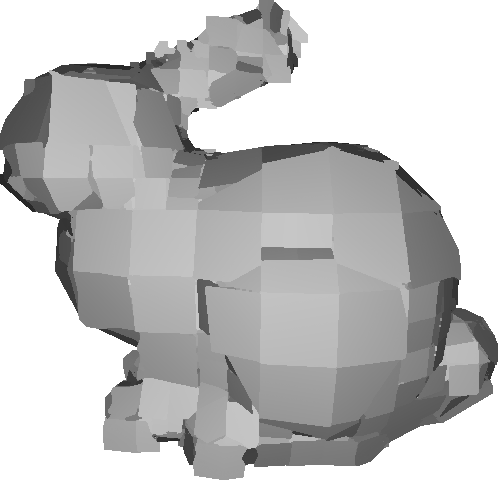
\includegraphics[width=1.8in]{images/experiments/pt_qual/planetree2_shade}
                \captionsetup{justification=centering}
                \caption{Plane-Tree\\0.31 bpv\\1,349 bytes}
                \label{fig:PT_SOTAQ1_PLT}
        \end{subfigure}%
        \begin{subfigure}[b]{2in}
                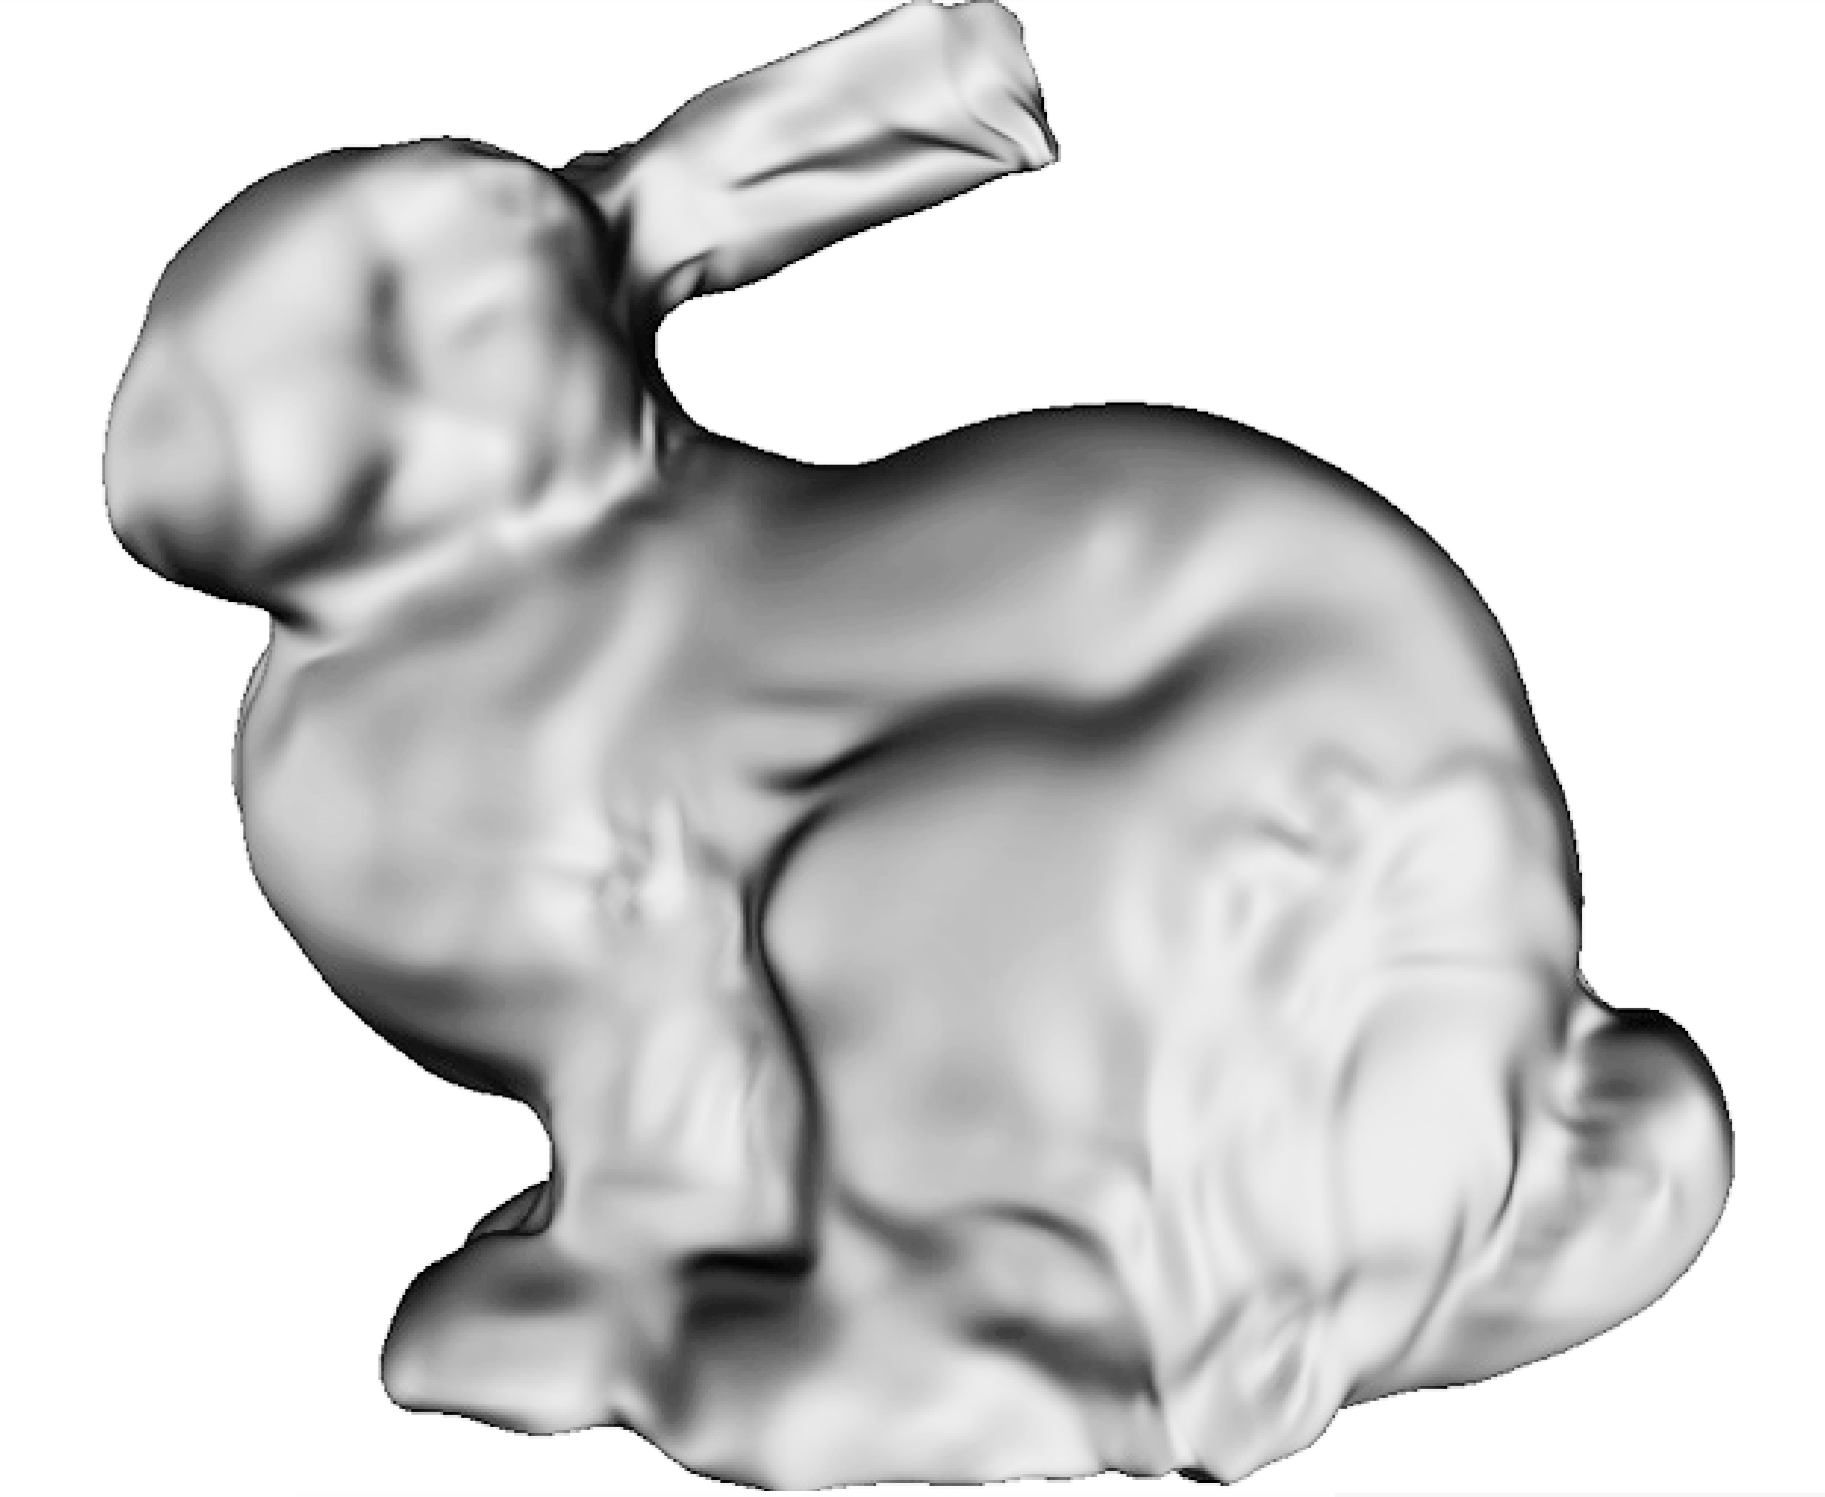
\includegraphics[width=1.8in]{images/experiments/pt_qual/khodakovsky_shade}
                \captionsetup{justification=centering}
                \caption{Khodakovsky et al. \cite{Khodakovsky00Progressive}\\0.31 bpv\\1,349 bytes}
                \label{fig:PT_SOTAQ1_KHKY}
        \end{subfigure}
       \caption{The Bunny Model Compressed Using the Plane-Tree and the Wavelet Compression System Khodakovsky et al.}
       \label{fig:qualSOTA2}
       \end{center}
\end{figure}

